\documentclass{aa}
\usepackage[varg]{txfonts}
\usepackage[separate-uncertainty=true]{siunitx}
\usepackage[version=3]{mhchem}

\sisetup{range-units = brackets}

\def\eps{\varepsilon}
\def\aap{A\&A}
\def\eprint{e-prints}
\def\apj{ApJ}
\def\apjs{ApJS}
\def\apjl{ApJL}
\def\mnras{MNRAS}
\def\aj{AJ}
\def\nat{Nature}
\def\aaps{A\&A Supp.}
\def\prd{Phys. Rev. D}
\def\prl{Phys. Rev. Lett.}
\def\araa{ARA\&A}       % Annual Review of Astron and Astrophys

\begin{document}


\title{NIR spectroscopy of the Sun and HD20010}
\subtitle{Compiling a new linelist in the NIR}


\author{ D.~T.~Andreasen\inst{1,2}
    \and S.~G.~Sousa.\inst{1,2}
    \and E.~Delgado Mena.\inst{1,2}
    \and N.~C.~Santos.\inst{1,2}
    \and M.~Tsantaki.\inst{1,2}
    \and B.~Rojas-Ayala.\inst{1}
    \and V.~Neves.\inst{3}}


\institute{
Instituto de Astrof\'isica e Ci\^encias do Espa\c{c}o, Universidade do Porto, CAUP, Rua das Estrelas, PT4150-762 Porto, Portugal
\email{daniel.andreasen@astro.up.pt}
\and
Departamento de F\'isica e Astronom\'ia, Faculdade de Ci\^encias, Universidade do Porto, Portugal
\and
Departamento de F\'{i}sica, Universidade Federal do Rio Grande do Norte, 59072-970 Natal, RN, Brazil
}





\date{Received ...; accepted ...}

\abstract
% Context
{Effective temperature, surface gravity, and metallicity are basic
spectroscopic stellar atmospheric parameters necessary to characterize
a star or a planetary system. Reliable atmospheric parameters for
FGK stars have been obtained mostly from methods that relay on high
resolution and high signal to noise optical spectroscopy. With the
advent of a new generation of high resolution near-IR spectrographs,
opens the possibility of using classic spectroscopic methods with
high resolution and high signal-to-noise in the NIR spectral window.}
% Aims
{We aim to compile a new iron line list in the NIR from a solar
spectrum, to derive precise stellar atmospheric parameters,
comparable to the ones already obtained from high resolution optical
spectra. The spectral range will be from \SI{10000}{\angstrom} to
\SI{25000}{\angstrom}.}
% Methods
{Our spectroscopic analysis is based on the iron excitation and
ionization balance done in LTE. The abundance analysis was done using
the MOOG code after measuring equivalent widths of 357 iron lines. We
use a high resolution and high signal-to-noise ratio spectrum of the Sun
from the Kitt Peak telescope as a starting point to compile the iron
line-list. The oscillator strengths were calibrated for the Sun.}
% Results
{We successfully derived stellar atmospheric parameters for the
Sun. With added noise to the EW measurements, to simulate a lower
signal-to-noise, of the Sun we re-derived parameters in perfect
agreement with the calibrated line-list. Furthermore, we analysed
HD20010, a F8IV star, from which we derived stellar atmospheric
parameters. The spectrum was obtained from the CRIRES-POP database. We
were not able to measure all iron lines in the spectrum of HD20010. In
some cases they were not present while in other cases they were blended
with either other elements or tellurics. With the lack of \ion{Fe}{ii}
lines from the spectrum we used, we were not able to derive the surface
gravity, which was fixed during the process.}
% Conclusions
{}



\keywords{data reduction: high resolution spectra --
          stars individual: HD20010 --
          stars individual: Sun}
\maketitle



\section{Introduction}
\label{sec:introduction}

Effective temperature ($T_\mathrm{eff}$), surface gravity ($\log g$),
and metallicity ([Fe/H], where iron is normally used as a proxy)
are fundamental atmospheric parameters necessary to characterise a
star, as well as to determine other indirect fundamental parameters,
such as mass, radius, and age from stellar evolutionary models
\citep[e.g.][]{Girardi2000,Dotter2008,Baraffe2015}.

Precise and accurate stellar parameters are also essential in
exoplanet searches. Planetary radius and mass are mainly found from
lightcurve analysis and radial velocity analysis, respectively. The
determination of the mass of the planet implies a knowledge of the
stellar mass, while the measurement of the radius of the planet
is dependent on our capability to derive the radius of the star
\citep{Ammler2009,Torres2008,Torres2012}.

The derivation of precise stellar atmospheric parameters is not a simple
task. Different approaches often lead to discrepant results \citep[see
e.g.][]{Santos13}. Interferometry is usually considered as an accurate
method to derive stellar radii \citep[e.g.][]{Boyajian2012}, however,
is only applicable for bright nearby stars. Asteroseismology, on the
other hand, reveals the inner stellar structure by observing the stellar
pulsations at the surface. From asteroseismology it is possible to
measure the surface gravity and mean density, and therefore calculate
the mass and radius \citep[e.g.][]{Kjeldsen1995}. Asteroseismology has
been tested to great extent with e.g. \emph{Kepler} and \emph{CoRoT}
\citep{Michel2008,Huber2011,Huber2012}. \cite{Campante2015} is a recent
example of usage of asteroseismology for characterization of planetary
system.

A key to all these approaches is a correct determination of the
effective temperature. In that respect, the IRFM is usually
considered as one of the most reliable methods for FGK dwarf
and subgiant stars. However, the IRFM needs a priori knowledge
of the bolometric flux, surface gravity and stellar metallicity
\citep{Blackwell1977,Ramirez2005b,Casagrande2010}.

Finally, the use of high resolution spectroscopy along with stellar
atmospheric models is an extensively tested method that allows
the derivation of the fundamental parameters of a star \citep[see
e.g.][]{Santos13} The procedure depends on the quality of the spectra,
their resolution, and wavelength region. For low resolution spectra
($\lambda/\Delta\lambda < 20\,000$) it is preferred to fit the overall
observed spectrum with a synthetic one \citep[see e.g.][]{Recio2006}.
For higher resolution spectra of slowly rotating stars (below 10 to 15
\si{km/s}) we are in the regime where the equivalent width (EW) method
can be used (for details see Sect.~\ref{sec:method}).

The derivation of stellar atmospheric parameters from high
resolution spectra in the optical is now based on a standard
procedure \citep[see e.g.][]{Valenti2005,Sousa2008a}. With the
advancement of NIR instruments, we will now be able to use a similar
technique as used in the visible part of the spectrum \citep[see
e.g.][]{Melendez1999,Tsantaki2013,Sousa2008a,Bensby2014,Mucciarelli2013}
. At the moment the GIANO spectrograph installed at TNC is already
available \citep{GIANO}, as well as the IRD spectrograph installed at
Subaru \citep{IRD}. Three new spectrographs are planned for the near
future: 1) CRIRES+ at VLT \citep{CRIRESp} with expected first light in
2017, 2) CARMENES for the 3.5 m telescope at Calar Alto Observatory
\citep{CARMENES} with expected first light at December 2015, and 3)
SPIRou at CFHT \citep{SPIROU1,SPIROU2} with expected first light in 2017
as well. The spectral resolutions for these spectrographs range between
$50\,000$ and $100\,000$.

Even though reliable line lists for the derivation of stellar parameters
using optical spectra exist, the situation is different in the near-IR
regime. In this paper we thus want to explore the possibility to create
a line list of iron lines in the NIR which can be applied for FGK stars
in a consistent way as it is currently done for these stars in the
optical. The paper is organized as follows: In Sect.~\ref{sec:method}
we present the method for deriving parameters with the equivalent width
method for an iron line list. In Sect.~\ref{sec:results} we present the
results for the derived parameters for the Sun and HD20010.




\section{Method}
\label{sec:method}

The two most widely used methods for deriving stellar atmosphere
parameters from a spectrum are spectral synthesis and the equivalent
width method. The spectral synthesis method compares synthetic spectra
to an observed spectrum and finds the best model by a minimization
procedure \citep[see e.g.][]{Valenti2005,Onehag2012,Blanco2014}. When
the minimization procedure reaches a minimum, the final atmospheric
parameters are found.

The equivalent width (EW) method
\citep{Sousa2008a,Bensby2014,Mucciarelli2013}, which we use in this
work, is based on the measurements of EWs of a given line list of atomic
data of absorption lines visible in the stellar spectrum of interest.
The EW for a single line is given as:
\begin{align}
    \label{eq:EW}
    EW = \int_0^\infty \left(1 - \frac{F_\lambda}{F_0}\right) d\lambda,
\end{align}
where $F_0$ is the continuum level and $F_\lambda$ is the flux as a
function of wavelength.

Using the EW method, the abundance for individual lines can be
calculated with a LTE excitation and ionization transfer code like
MOOG \citep{Sneden1973}. By changing atmospheric parameters in the
input model for MOOG, we expect to retrieve the same abundances for
every spectral line of the same element when the best atmospheric
parameters are chosen. Here we use neutral iron and single ionized
iron: \ion{Fe}{i} and \ion{Fe}{ii}, respectively, which are also used
to fix the surface gravity by achieving ionization balance. This allows
us to derive stellar parameters using the principle of ionization and
excitation equilibrium \citep{Gray2006}.

A disadvantage of the EW method, is the determination of the continuum
flux level, since a misplacement of the continuum level leads to an
over- or underestimation of the EW for a given line. In this work we
will focus at the spectral region covered by the J, H, and K bands,
which covers more than $\SI{15000}{\AA}$.



\subsection{Compiling the line list}

To compile the line list we use the VALD3 database \citep{VALD1,VALD2}.
First we download all iron lines present in the near infrared
region, covering $10\,000\si{\AA}$ to $25\,000\si{\AA}$. In
total, $78\,537$ iron lines were found in that spectral region
($50\,198$ \ion{Fe}{i} lines and $28\,339$ \ion{Fe}{ii} lines).
Many of these lines are too faint to be detected in the spectrum
of a solar type star. A spectrum of the Sun was downloaded from
the BASS2000 web page\footnote{The web page can be found here:
\url{bass2000.obspm.fr/solar_spect.php}} to select the lines. The
NIR part of the spectrum downloaded from this web page were obtained
from the Kitt Peak telescope \citep{Hinkle1995} at a resolution of
\SI{0.004}{\angstrom} at \SI{10000}{\angstrom} to \SI{0.1}{\angstrom}
at \SI{50000}{\angstrom}. The spectrum was downloaded in the highest
possible resolution. The signal-to-noise ratio of the spectrum varies
from 3000 at $\SI{12000}{\AA}$ down to 1400 at $\SI{21400}{\AA}$. We
use the ARES software\footnote{The ARES software can be found here:
\url{http://www.astro.up.pt/~sousasag/ares/}}\citep{Sousa2007,Sousa2015a
} to automatically measure EWs of all the lines. Since the first version
of ARES expect a 1D spectrum with equidistant wavelength spacing,
the solar spectrum was interpolated to a regular grid with constant
wavelength step of \SI{0.01}{\angstrom}. The EWs are measured by fitting
Gaussian profiles to spectral lines. For a given line ARES outputs the
central wavelength of the line, the number of lines fitted for the end
result, the depth of the line, the FWHM of the line, the EW of the line,
and Gaussians coefficients for the line.

Once this step is done we then selected a subset of lines using the
following criteria:
\begin{itemize}
    \item If the number of fitted lines by ARES for a given line is higher than 10,
        this line is rejected because it is believed to be severely blended.
    \item If the EW is lower than \SI{5}{m\angstrom} for an absorption line, the strength
        is too low and may be difficult to see it in spectra with low S/N or a
        spectrum with many spectral features.
    \item If the EW is higher than \SI{200}{m\angstrom} for a given line, the strength
        is too high and we can no longer fit the line with a Gaussian profile.
    \item If the fitted central wavelength is more than $\SI{0.05}{\AA}$ away
        from the wavelength provided by VALD3, the line will also be rejected to
        avoid false identification.
\end{itemize}
After the automatic removal of lines following the above criteria
we reduced the number of lines to 6060 and 2735 for \ion{Fe}{i} and
\ion{Fe}{ii}, respectively.



\subsection{Visual removal of lines}
\label{sub:visual_removal_of_lines}

A visual inspection of the lines is necessary at this point in order to
allow us to select only the best lines.

In this step we analyzed in detail small \SI{3}{\angstrom} wide spectral
windows around each line. For each spectral window, the corresponding
absorption lines for all elements were downloaded from the VALD3 data
base. The location of these lines were plotted on top of the solar
spectrum, and iron lines were excluded when a line of another element
was present at the same wavelength. Iron lines were also excluded when
the absorption line was severely blended by other spectral lines. Many
of the removed iron lines at this step have high excitation potential,
compared to the final line list, since these lines are generally weaker
than those with lower excitation potential. After this step we were down
to 593 \ion{Fe}{i} lines and 22 \ion{Fe}{ii} lines.

For some spectral regions it was not clear which element or elements
caused an absorption line. In these cases the iron lines were marked for
further investigation with synthesis explained below.


\subsection{Synthesis of selected lines}
\label{sub:synthesis_of_selected_lines}

Lines from all elements in a $\SI{6}{\AA}$ window around an iron line
marked for further investigation were used to make a synthetic spectrum.
The synthetic spectra were made with MOOG with the synth driver. The
atmosphere model is a ATLAS9 atmosphere model \citep{Kurucz1993} with
the following atmospheric parameters: $T_\mathrm{eff}=\SI{5777}{K}$,
$\log g = 4.438$, and $\xi_\mathrm{micro} = \SI{1.0}{km/s}$ to resemble
the Sun. We used 3 different iron abundances for the synthesis. One
with solar iron abundance, the second with 0.2 dex above solar and the
third with 0.2 dex below solar. We consider a solar iron abundance
of 7.47 as found in \cite{Gonzalez2000}. If the synthetic spectra
shows variation at the absorption line of interest with respect to the
different iron abundances, then it's likely to be an iron line. We also
changed abundances of other elements in the proximity to see if our line
is blended with other elements. An example of these plots can be seen in
Fig~\ref{fig:synthesis}.

\begin{figure}[tpb]
    \centering
    \includegraphics[width=1.0\linewidth]{figures/synthetic_spectrum.pdf}
    \caption{Top panel shows the observed spectra in grey, while
        the colored graphs is synthetic spectra with increasing iron
        abundance as the central two lines get deeper. The iron abundance
        is varied 0.4 dex in total. The vertical lines show all the places
        there are an iron line in the line list. Bottom panel shows
        two plots, namely the difference between the first synthetic curve
        and the second, and the third ($\Delta_{21}$ and $\Delta_{31}$,
        respectively). This is for highlighting where the change in iron
        abundance has an impact.}
    \label{fig:synthesis}
\end{figure}


Sometimes more than one iron line might be present with very similar
wavelengths. In order to find the iron line which is creating the
absorption line, one of the two were removed from the line list for
the synthetic spectra. If this removed (either fully or partially) the
absorption line in the synthetic spectra, then it will be the cause for
the real absorption line.

A few times two iron lines had identical wavelengths and excitation
potential. In those cases the $\log \mathit{gf}$ were combined (sum
of the gf-value) to create a single line that can be analyzed with
our method. We ended up with 593 and 12 lines of \ion{Fe}{i} and
\ion{Fe}{ii}, respectively.


\subsection{Calibrating the line-list: astrophysical $\log$ gf values}
\label{ssub:Recalibrating-the-atomic-data}

The iron abundances for each line were calculated using the same
solar atmosphere model as described above for synthesis. This step
allowed us to remove possible outliers based on the assumption that
errors in the $\log \mathit{gf}$ values from the VALD3 database
would never lead to variations of the derived iron abundance of more
than 1 dex. Note that we only removed \ion{Fe}{i} lines here, since
the \ion{Fe}{ii} lines are sparse and essential to determine the
surface gravity when we reach ionization balance, as explained in
Sect.~\ref{sec:deriving_parameters_with_the_ew_method}. At this point
we are down to 319 and 12 lines, for \ion{Fe}{i} and \ion{Fe}{ii}
respectively.

After the removal of lines from the complete VALD3 line list we
recalibrate the oscillator strength of the lines ($\log \mathit{gf}$)
in order to match the adopted solar abundance. This is one of the
ways to perform a differential analysis, which is a common thing
to do for a star we know well \citep{Sousa2008a,Onehag2012}. In
Fig~\ref{fig:Fe1_before_recal} the EWs of the iron lines present in
the Sun are plotted as a function of the excitation potential. This
plot shows the distribution after recalibration of $\log gf$ and cut
for lines with abundances deviating more than 1 dex from the solar
value. The majority of the iron lines are found in H band as shown in
Fig~\ref{fig:Fe1_after_recal}.



\begin{figure}[tpb]
    \centering
    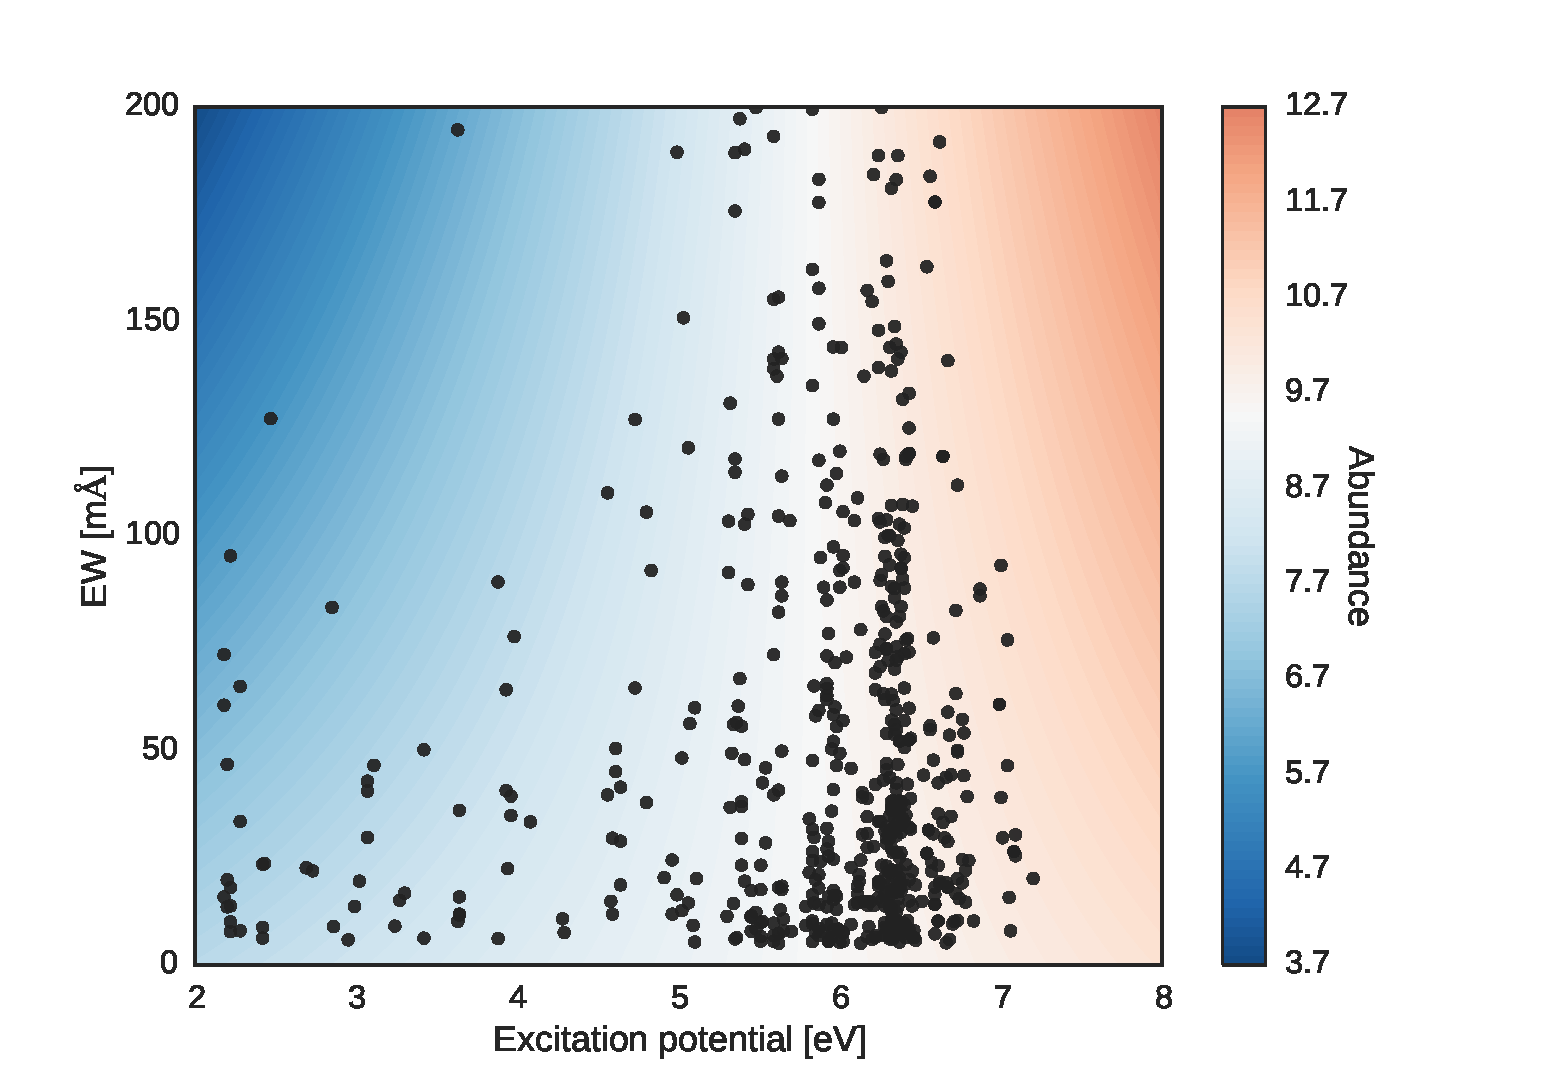
\includegraphics[width=1.0\linewidth]{figures/EWvsEP.pdf}
    \caption{The distribution of \ion{Fe}{i} and \ion{Fe}{ii} lines,
    colored blue and red, respectively. At the x axis is
    the excitation potential, while the measured EWs for the Sun is
    shown at the y axis.}
    \label{fig:Fe1_before_recal}
\end{figure}


\begin{figure}[tpb]
    \centering
    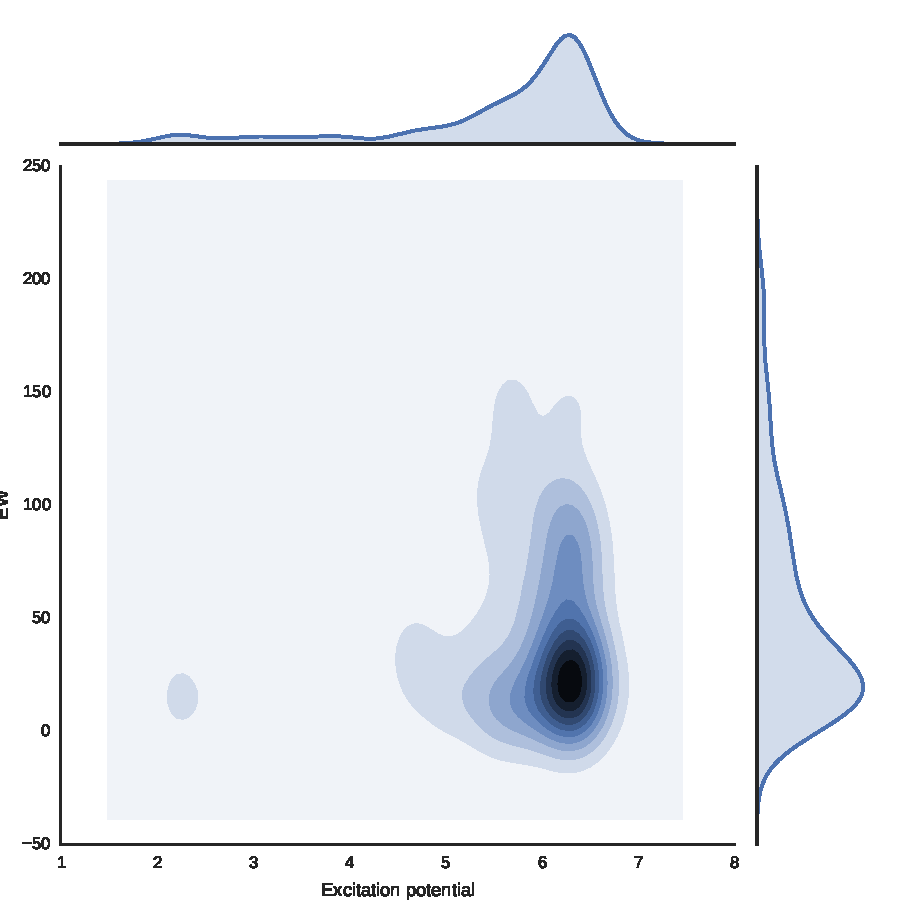
\includegraphics[width=1.05\linewidth]{figures/EWvsEP_cut.pdf}
    \caption{Distribution of both \ion{Fe}{i} and \ion{Fe}{ii} lines on top of the solar
    spectrum. The distributions are after recalibration and exclusion
    of lines which deviate more than 1 dex from the expected solar iron
    abundance. There are two areas in the spectrum with high telluric
    contamination, which also mark the border between the filters we
    use: from J to H around 14000\si{\angstrom} and from H to K around
    19000 \si{\angstrom}. Most of the lines are located in the H band.}
    \label{fig:Fe1_after_recal}
\end{figure}


\subsection{Removal of unstable lines}
\label{sub:removal_of_unstable_lines}

We want to check the stability of the lines selected at thie point. The
recipie for this is very simple. A gaussian distribution is made for the
EW of each line following the formula presented in \citet{Caryel1988}
presented below.

\begin{align}
    \sigma \simeq 1.6 \frac{\sqrt{\Delta\lambda\; \mathrm{EW}}}{\mathrm{S/N}},
\end{align}
where $\Delta\lambda=0.1\si{\angstrom}$ and we consider a
signal-to-noise ratio of 50, much lower than the signal-to-noise ratio
of the spectrum. This sigma is used to create a normal distribution with
a mean around the original EW.
\begin{align}
    f(x, EW, \sigma) = \frac{1}{\sqrt{2\pi\sigma^2}} e^{-\frac{(x-EW)^2}{2\sigma^2}}.
\end{align}
We make 100 draws and derive the abundance for each line with Solar
parameters, using the same atmospheric model as described above. The
mean absolute deviation (MAD) is calculated for all lines and plotted
against the EW, since low EW will naturally have higher MAD values. The
curve is detrended with an exponential function, and from the residuals
we iteratively remove the point furthest away above $3\sigma$. In this
process 23 lines are removed as shown in Fig.~\ref{fig:unstable_lines}.

\begin{figure}[tbp!]
    \centering
    \includegraphics[width=1.0\linewidth]{figures/unstable_lines.pdf}
    \caption{The upper plot shows the MAD values of 100 noisy lines with
    a simulated signal-to-noise ratio of 30. The red points are the 23
    detected unstable lines, and the red curve is the last fit in the
    iterative removal of unstable lines.
    The lower plot show the detrended points from the upper plot, from
    where the $3\sigma$ is calculated for each iteration.}
    \label{fig:unstable_lines}
\end{figure}

The final line list is presented in Tab.~\ref{tab:linelist}

\begin{table*}[tb!]
    \caption{The final line list as found for the Sun.}
    \label{tab:linelist}
    \centering
    \begin{tabular}{lllll}
      \hline\hline
        Wavelength &  Element      &  Excitation potential & $\log\mathit{gf}$ &    EW   \\
      \hline
        10070.521  &   \ion{Fe}{i} &          5.51         &        -1.527     &     6.6 \\
        10080.415  &   \ion{Fe}{i} &          5.10         &        -2.008     &     5.3 \\
        10081.394  &   \ion{Fe}{i} &          2.42         &        -4.551     &     6.2 \\
        10086.242  &   \ion{Fe}{i} &          2.95         &        -4.059     &     5.8 \\
        10137.100  &   \ion{Fe}{i} &          5.09         &        -1.768     &     9.2 \\
        10142.844  &   \ion{Fe}{i} &          5.06         &        -1.574     &    14.4 \\
        10155.163  &   \ion{Fe}{i} &          2.18         &        -4.340     &    15.8 \\
        10156.507  &   \ion{Fe}{i} &          4.59         &        -2.125     &    11.8 \\
        10167.469  &   \ion{Fe}{i} &          2.20         &        -4.199     &    19.8 \\
        10195.106  &   \ion{Fe}{i} &          2.73         &        -3.625     &    21.9 \\
        10198.427  &   \ion{Fe}{i} &          6.02         &        -1.152     &     5.4 \\
        10227.991  &   \ion{Fe}{i} &          6.12         &        -0.449     &    19.4 \\
        10230.796  &   \ion{Fe}{i} &          6.12         &        -0.414     &    21.0 \\
        10265.218  &   \ion{Fe}{i} &          2.22         &        -4.668     &     7.7 \\
        10283.776  &   \ion{Fe}{i} &          5.51         &        -1.621     &     5.5 \\
        10307.450  &   \ion{Fe}{i} &          4.59         &        -2.500     &     5.5 \\
        10327.340  &   \ion{Fe}{i} &          5.54         &         0.504     &   134.4 \\
        10332.328  &   \ion{Fe}{i} &          3.63         &        -3.145     &    10.1 \\
        10347.966  &   \ion{Fe}{i} &          5.39         &        -0.754     &    36.9 \\
        10353.805  &   \ion{Fe}{i} &          5.39         &        -1.035     &    23.2 \\
        10364.063  &   \ion{Fe}{i} &          5.45         &        -1.129     &    17.3 \\
        10379.000  &   \ion{Fe}{i} &          2.22         &        -4.246     &    18.0 \\
        10388.746  &   \ion{Fe}{i} &          5.45         &        -1.527     &     7.8 \\
        10423.029  &   \ion{Fe}{i} &          2.69         &        -3.660     &    22.6 \\
        \ldots     &   \ldots      &          \ldots       &        \ldots     &   \ldots\\
        10427.305  &  \ion{Fe}{ii} &          6.08         &        -1.662     &    12.4 \\
        10501.498  &  \ion{Fe}{ii} &          5.55         &        -1.926     &    18.2 \\
        10862.644  &  \ion{Fe}{ii} &          5.59         &        -2.043     &    14.8 \\
        11125.580  &  \ion{Fe}{ii} &          5.62         &        -2.301     &     9.1 \\
        11833.056  &  \ion{Fe}{ii} &          2.84         &        -3.379     &    81.7 \\
        12913.876  &  \ion{Fe}{ii} &          6.50         &         0.045     &    97.7 \\
        13251.144  &  \ion{Fe}{ii} &          9.41         &         0.860     &    13.0 \\
        13277.306  &  \ion{Fe}{ii} &          5.29         &        -2.043     &    35.9 \\
        13294.853  &  \ion{Fe}{ii} &          3.22         &        -3.613     &    56.9 \\
        13419.109  &  \ion{Fe}{ii} &          3.81         &        -3.484     &    32.8 \\
        15247.133  &  \ion{Fe}{ii} &          6.84         &        -1.691     &    10.5 \\
        15350.156  &  \ion{Fe}{ii} &          8.95         &         0.602     &    29.0 \\
        20460.070  &  \ion{Fe}{ii} &          1.67         &        -5.758     &    36.5 \\
      \hline
    \end{tabular}
\end{table*}



\subsection{Deriving parameters with the EW method}
\label{sec:deriving_parameters_with_the_ew_method}

Once the EWs have been measured for all lines in the line list (or as
many as possible), the next step is to derive atmospheric parameters.
Atmosphere models are necessary for computing abundances of the lines.
The literature offers the possibility to choose from a wide variety
of model atmospheres. Models like ATLAS9 \citep{Kurucz1993} and
MARCS \citep{Gustafson2008} are the most used atmospheric models for
derivation of spectroscopic parameters for FGK stars.

Here we use the ATLAS9 models which, for efficiency, are created
in a grid according to effective temperature, surface gravity, and
metallicity. In order to search for final parameters it is necessary to
interpolate models from the grid, thus allowing to look into a finer
grid space \citep[see e.g.][]{Sousa2014}.

For a given atmosphere model, abundances of all the lines in the line
list are calculated. By removing any correlation between the excitation
potential and abundance of all lines (from same element) the effective
temperature is constrained. In a similar way, the micro turbulence
can be constrained be removing any correlation between the reduced EW
($\log EW/\lambda$) and iron abundances, and the surface gravity is
found when there is ionization balance, i.e. the mean abundance of
\ion{Fe}{i} and \ion{Fe}{ii} are equal. Lastly, the iron abundance comes
from calculating the mean of all the iron abundances.

When there are no longer any correlation, the final atmospheric
parameters are obtained from the atmospheric model to calculate the
given abundances.

In order to find the best atmosphere model, a minimization algorithm
is used based on the downhill simplex method \citep{Press1992}
that searches in the parameter space for the best fitting model.
The convergence criteria for the correlation between excitation
potential and abundances gives a slope less than 0.001, a slope
less than 0.002 for the correlation between the reduced EW and
the abundances, and a difference of less than 0.005 between the
mean abundances for \ion{Fe}{i} and \ion{Fe}{ii} as used in e.g.
\citet{Tsantaki2013,Sousa2008a}.







\section{Results}
\label{sec:results}


\subsection{Derived parameters for the Sun}
\label{sec:derived_parameters_of_the_sun}

As a test, we then derived the stellar parameters for the Sun using
the resulting line-list (including the solar calibrated, astrophysical
$\log \mathit{gf}$ values). We used the minimization procedure described
in Sect.~\ref{sec:deriving_parameters_with_the_ew_method}. Since the
line-list and $\log\mathit{gf}$ values have been selected using the
solar spectrum, it is with no surprise that the derived parameters for
the Sun perfectly match the adopted solar values within the error bars.

Moreover we derive parameters for different signal-to-noise ratios,
namely 10, 25, 50, 100, 150, and 300. The signal-to-noise ratios
are obtained by drawing EW from a gaussian distribution with widths
dependent on the EW itself and the signal-to-noise as described above
in Sec.\ref{sub:removal_of_unstable_lines}. For each signal-to-noise we
consider we make 10 line lists, giving us a total of 60 line lists. This
exercise show the expected precision we for different signal-to-noises,
with the presented line list. The final results are presented in
Fig.\ref{fig:snr_sun}. The error is the $3 \sigma$ standard deviation
from the 10 different runs. As seen from the figure, we expect to
be able to derive precise parameters, (effective temperature more
precise than $\SI{50}{K}$, surface gravity to a precision of 0.1 dex,
iron abundance to a precision of 0.05, and microturbulence down to a
precision of 0.3) down to a signal-to-noise ratio of 50. At higher
signal-to-noise ratios the precision generally increase. The results can
also be seen in Tab.~\ref{tab:solar_params}

\begin{figure*}[tbp!]
    \centering
    \includegraphics[width=1.0\linewidth]{figures/solar_parameters_snr.pdf}
    \caption{All plots shows derived parameters as a function of the
    signal-to-noise. The error is the 3$\sigma$ standard deviation from
    the 10 different runs for each signal-to-noise. The upper left plot
    shows the effective temperature. The upper right plot show the surface
    gravity ($\log g$). The lower left shows the iron abundance, used as a
    proxy for the metallicity. Finally, in the lower right plot is shown
    the microturbulence.}
    \label{fig:snr_sun}
\end{figure*}

\begin{table*}[htb!]
    \caption{The derived parameters for the Sun at different signal-to-noise
    ratios. The error is the 3$\sigma$ standard deviation calculated from
    the 10 runs at each signal-to-noise ratio.}
    \label{tab:hd20010}
    \centering
    \begin{tabular}{lllll}
      \hline\hline
        SNR & $T_\mathrm{eff}$ (K) & $\log g$ (cgs)  &       [Fe/H]     & $\xi_\mathrm{micro}$ (km/s)  \\
      \hline
        10  &    $5874 \pm 429$    & $4.92 \pm 0.20$ & $-0.05 \pm 0.13$ &     $4.75 \pm 2.05$          \\
        25  &    $5795 \pm 89$     & $4.52 \pm 0.20$ & $-0.01 \pm 0.04$ &     $1.34 \pm 0.52$          \\
        50  &    $5781 \pm 46$     & $4.45 \pm 0.08$ & $ 0.00 \pm 0.03$ &     $1.04 \pm 0.22$          \\
       100  &    $5784 \pm 25$     & $4.44 \pm 0.04$ & $ 0.00 \pm 0.01$ &     $1.02 \pm 0.11$          \\
       150  &    $5779 \pm 17$     & $4.43 \pm 0.04$ & $-0.00 \pm 0.03$ &     $1.03 \pm 0.17$          \\
       300  &    $5776 \pm 10$     & $4.43 \pm 0.01$ & $ 0.00 \pm 0.00$ &     $0.99 \pm 0.08$          \\
      \hline
    \end{tabular}
\end{table*}

Not all 60 runs converged. For the case with signal-to-noise ratio at
10, only 1 out of 10 of the line lists were able to converge with our
minimization routine. Additionally, 1 line list at signal-to-noise ratio
at 150 did not converge. However, they are all part of the analysis,
since the minimization routine returns the best stellar atmospheric
parameters for a given line list.




\subsection{Derived parameters for HD20010}
\label{sec:derived_parameters_of_hd20010}

For testing our new line list we need a well studied star with
parameters which resembles the Sun. The spectrum for such a target
needs to be available in the NIR at both high resolution and
signal-to-noise. An ideal place to look for such a star is the
CRIRES-POP database \citep{Lebzelter2012}. Here the best target for
testing is HD20010, a F8 subgiant star. This star have been part of
many surveys and are therefore well studied. \cite{Mortier2013} found
[Fe/H]=-0.19 from the cross-correlation function calibation, and
$T_\mathrm{eff}=\SI{6114}{K}$ from $B-V$ colour. \cite{Gonzalez2010}
found $T_\mathrm{eff} = 6170\pm35\si{K}$, $\log(g) = 3.93\pm0.02$ dex,
$\xi_\mathrm{micro} = 1.70\pm0.09\si{km/s}$, and [Fe/H]=$-0.206\pm0.025$
using the EW method with an optical spectrum. \cite{Balachandran1990}
found $T_\mathrm{eff} = 6152\si{K}$, $\log(g) = 4.15$ dex,
$\xi_\mathrm{micro} = 1.6\si{km/s}$, and [Fe/H]=$-0.27\pm0.08$ obtained
from Str\"{o}mgren \emph{uvby} H$\beta$ indices. \cite{Favata1997} found
$T_\mathrm{eff}=\SI{6000}{K}$ and [Fe/H] = $-0.35\pm0.07$ using the EW
method as well with 9 lines. \cite{Ramirez2012} found $T_\mathrm{eff}
= 6073\pm78\si{K}$, $\log(g) = 3.91\pm0.03$ dex, and [Fe/H] =
$-0.30\pm0.05$. The effective temperature from the latter result was
calculated from a colour-$T_\mathrm{eff}$ calibration, the metallicity
from analysis of both neutral and singly ionized iron lines, and the
surface gravity was derived from mass estimates based on theoretical
isohcornes analysis and trigonometric \emph{Hipparcos} parallaxes. The
above works are just few of many studies of this star. We compare our
result for this star with the mean of the above mentioned results,
which yield: $T_\mathrm{eff} = 6101\si{K}$, $\log(g) = 4.00$ dex,
$\xi_\mathrm{micro} = 1.65\si{km/s}$, and [Fe/H]=$-0.26$.

The data available at CRIRES-POP is currently pipeline reduced, while
three small pieces of the spectra of the spectra are fully reduced on
the web page\footnote{\url{http://www.univie.ac.at/crirespop/data.htm}}.
We measured the EW of the pipeline reduced spectra, and where there
was an overlap with the fully reduced spectrum, we measured as a
consistency check. The measured EWs showed good agreement in the cases
where an overlap was present. As mentioned above, we use the J, H,
and K bands which are all available for this star. The spectra comes
in pieces of $\SI{50}{\angstrom}$ to $\SI{120}{\angstrom}$. These
chunks have overlaps between each other, and usually we were able
to measure the EW for a single line up to five times, while between
three and four measurements were normal. Unfortunately, wavelength
calibration is a difficult task for CRIRES due to the rather small
spectral regions measured on each detector. Each calibration was
performed separately for each detector and required the availability
of a sufficient number of calibration lines in the respective spectral
region. This was not always the case and a default linear solution
was applied. The wavelength calibration might be improved with the
usage of telluric lines. With the pipeline reduced spectra the
sometimes poor wavelength calibration is shown as a stretched spectrum
compared to e.g. a model spectrum or a solar spectrum. The pipeline
reduced spectra for HD20010 contains tellurics and are shifted with a
radial velocity. All this combined make the line identification very
difficult. Therefor we developed a software\footnote{The software
(plot\textunderscore{}fits) is open source and can be found here:
\url{https://github.com/DanielAndreasen/astro_scripts}} to help us. This
software does the following:
\begin{enumerate}
    \item Plot the observed spectrum.
    \item Over plot a model spectrum. In this particular the solar spectrum was
        used since the atmospheric parameters are close enough, so the sun can
        serve as a model.
    \item Over plot a telluric spectrum from the TAPAS web page \citep{Bertaux2014}.
    \item Over plot a vertical line at the location for lines in the list.
    \item Calculate the cross correlation function (CCF) for the telluric spectrum
        respect to the observed spectrum, locate the maximum value by a Gaussian fit
        and use this to shift the telluric spectrum with the found RV.
    \item Do the same as the step above, but for the model.
\end{enumerate}
The final plot shows the shifted spectra, and the CCFs at the sides. An
example of the software in use is shown in Fig.~\ref{fig:plot_fits}. The
two RVs are part of the title of the plot.



\begin{figure*}[tbp!]
    \centering
    \includegraphics[width=1.0\linewidth]{figures/plot_fits.pdf}
    \caption{The middle plot shows a piece of HD20010 (black), the model
    spectrum, in this case the Sun (green), a telluric spectrum (red), and two
    lines from our line list (magenta vertical lines). The plot to the left
    shows the CCF of the Sun with a fitted Gaussian. The right plot shows the
    same as the one to the left, but for the telluric spectrum.}
    \label{fig:plot_fits}
\end{figure*}

Once the lines are identified the EWs were measured with the splot
routine in IRAF. The reason not to choose ARES for this task was to
visually confirm the identification of the line given the relative
poor wavelength calibration at the moment. We were able to measure 249
\ion{Fe}{i} lines and 5 \ion{Fe}{ii} lines compared to 344 \ion{Fe}{i}
lines and 13 \ion{Fe}{ii} lines for the Sun over the whole NIR spectral
region.

We then derived the stellar parameters using the standard procedure
(see Sect.~\ref{sec:deriving_parameters_with_the_ew_method}) as
done for the Sun. The final derived parameters for the full line
list are overestimated compared to literature values listed above.
Therefore, since the spectrum for HD20010 is not corrected for
telluric contamination, we make four cuts in EW and remove lines below
this threshold before deriving parameters again. Since the relative
affect by tellurics are larger for weak lines we expect to obtain
parameters in better agreement with the litterature. However, a too
high cut start to remove valuable information from the analysis, and
therefore we expect worse results. This is exactly was is presented in
Tab.~\ref{tab:hd20010} and Fig.~\ref{fig:HD20010_parameters_cuts}. We
choose to cut at 5, 10, 15, and 20 \si{m\angstrom} respectively. The
agreement with litterature is best at a cut at $\SI{15}{m\angstrom}$
where we have removed lines affected by blends with tellurics.


\begin{table*}[htb!]
    \caption{The derived parameters for HD20010 at different EW cut. $\log g$
        were fixed at 4.00 for all calculations.}
    \label{tab:hd20010}
    \centering
    \begin{tabular}{lllll}
      \hline\hline
        EW cut (\si{m\angstrom}) & $T_\mathrm{eff}$ (K) & $\xi_\mathrm{micro}$ (km/s) & [Fe/H]             \\
      \hline
        Literature               & $6101        $       & $1.65         $             & $-0.26         $   \\
      \hline
        No cut                   & $6417 \pm 153$       & $5.03 \pm 0.06$             & $-0.17 \pm 0.36$   \\
        5.0                      & $6437 \pm 209$       & $5.00 \pm 0.23$             & $-0.16 \pm 0.65$   \\
       10.0                      & $6350 \pm 370$       & $5.00 \pm 1.39$             & $-0.17 \pm 2.35$   \\
       15.0                      & $6040 \pm 237$       & $4.49 \pm 0.35$             & $-0.17 \pm 0.22$   \\
       20.0                      & $5841 \pm 910$       & $5.00 \pm 4.10$             & $-0.20 \pm 2.58$   \\
      \hline
    \end{tabular}
\end{table*}



% \begin{figure}[tpb!]
%     \centering
%     \includegraphics[width=1.0\linewidth]{figures/HD20010_parameters_cuts.pdf}
%     \caption{Atmospheric parameters for HD20010. In the top panel is
%     the effective temperature. The middle panel is the iron abundance,
%     and the bottom panel is the micro turbulence. The parameters are
%     derived with different cuts in EW. Here the horizontal black lines
%     are literature values. The parameters for the full line list are
%     plotted to the right for all three plots.}
%     \label{fig:HD20010_parameters_cuts}
% \end{figure}




\section{Conclusion}

In this work, we present a new iron line list for the NIR. The quality
of the line list plays a key role for deriving atmospheric stellar
parameters. While the line list was compiled from a solar spectrum and
calibrated for the same, we tested it extensively for the slightly
hotter star, HD20010. The first results with this line list are
promising. We also show that for a spectrum that contain telluric
lines best results appear when removing lines with a low EW around
$\SI{15}{m\angstrom}$.

The line list still remains to be tested for a larger sample of FGK
stars. Furthermore, it will be interesting to explore the use of this
line-list to derive parameters for M-dwarf stars using high resolution
and high S/N NIR spectra. M-dwarf stars are especially interesting
targets for an exoplanetary viewpoint, since they are prone to form
low mass exoplanets \citep{Bonfils2013}. Hence, a precise analysis
of the host star's atmospheric parameters may greatly improve our
characterization of the possible exoplanets orbiting these low mass
stars.

Lastly, with the up-coming NIR spectrographs, this work and future
continuation will help the community to derive atmospheric stellar
parameters.





\begin{acknowledgements}

This work was supported by Funda\c{c}\~ao para a Ci\^encia e a
Tecnologia (FCT) through the research grant UID/FIS/04434/2013.
E.D.M, P.F., N.C.S., and S.G.S. also acknowledge the support from FCT
through Investigador FCT contracts of reference SFRH/BPD/76606/2011,
IF/01037/2013, IF/00169/2012, and IF/00028/2014, respectively, and
POPH/FSE (EC) by FEDER funding through the program “Programa
Operacional de Factores de Competitividade - COMPETE”.

This research has made use of the SIMBAD database operated at CDS,
Strasbourg (France).

This work has made use of the VALD database, operated at Uppsala
University, the Institute of Astronomy RAS in Moscow, and the University
of Vienna.

\end{acknowledgements}






\bibpunct{(}{)}{;}{a}{}{,}
\bibliographystyle{aa}
\bibliography{thesis}

\end{document}
